\documentclass[tikz,border=6pt]{standalone}
% Shared preamble of the standalone figures: fonts as in the decks, the TikZ
% libraries, the notation, and the styles.
\usepackage[T1]{fontenc}
\usepackage[utf8]{inputenc}
\usepackage[sfdefault,lining]{FiraSans}
\usepackage{FiraMono}
\usepackage{amsmath}
\usetikzlibrary{positioning,arrows.meta,calc,shapes.misc,fit,backgrounds,
                decorations.pathreplacing,patterns,matrix}
% Notation for the MACE4D figures.
%
% Every parameter, symbol, default value, and constant that a figure shows is
% a macro here, so that the figures change from code names to symbols, or
% follow a change of a default, by editing this file alone.
%
%   \codenamestrue   renders each parameter as its code name (current setting)
%   \codenamesfalse  renders the symbolic form
%
% \sym{code name}{symbol} is the switch every parameter macro uses.  A
% parameter that exists on both models carries its owner in code mode.

\newif\ifcodenames
\codenamestrue

\providecommand{\code}[1]{\texttt{#1}}
\newcommand{\sym}[2]{\ifcodenames\code{#1}\else\ensuremath{#2}\fi}
\newcommand{\ctmodel}{\code{ct\_model}}
\newcommand{\macemodel}{\code{MACE4DModel}}
% A key line "code name <-> symbol", shown in code mode only.
\newcommand{\keyline}[2]{\ifcodenames#1~\ensuremath{\leftrightarrow}~\ensuremath{#2}\fi}

% ------------------------------------------------------------ math symbols
% These are always symbolic; the formulas use them, and the key lines tie
% them to the code names.
\newcommand{\symSigY}{\sigma_y}
\newcommand{\symSigProx}{\sigma_p}
\newcommand{\symSigNoise}{\sigma_n}
\newcommand{\symSigX}{\sigma_x}
\newcommand{\symSharpness}{s}
\newcommand{\symBeta}[1]{\beta_{#1}}
\newcommand{\symRho}{\rho}
\newcommand{\symNbrWeightTime}{b_t}
\newcommand{\symNumFrames}{T}
\newcommand{\symFramesPerRotation}{P}
\newcommand{\symOverlap}{f}

% ------------------------------------------------------------------ objects
\newcommand{\frameCube}[1]{\ensuremath{C_{#1}}}          % frame t of the 4D image
\newcommand{\fourD}{\ensuremath{x}}                      % the 4D image
\newcommand{\initImage}{\ensuremath{x^{0}}}              % the initial 4D image
\newcommand{\sinoFrame}[1]{\ensuremath{y_{#1}}}          % the views of frame t
\newcommand{\weightsFrame}[1]{\ensuremath{\Lambda_{#1}}} % the weights of frame t
\newcommand{\projFrame}[1]{\ensuremath{A_{#1}}}          % the frame model
\newcommand{\proxAgent}[1]{\ensuremath{F_{#1}}}          % the prox map of frame t
\newcommand{\dataFitAgent}{\ensuremath{F}}               % all frames' prox maps as one agent
\newcommand{\orientXY}{\sym{XY-t}{\mathrm{XY}t}}
\newcommand{\orientYZ}{\sym{YZ-t}{\mathrm{YZ}t}}
\newcommand{\orientXZ}{\sym{XZ-t}{\mathrm{XZ}t}}
\newcommand{\denoiser}[1]{\ensuremath{G_{#1}}}           % \denoiser{\orientXY}
\newcommand{\stateW}[1]{\ensuremath{W_{#1}}}             % the loop's input to agent k
\newcommand{\outX}[1]{\ensuremath{X_{#1}}}               % the output of agent k
\newcommand{\avgZ}{\ensuremath{z}}
\newcommand{\xbar}{\ensuremath{\bar{x}}}
\newcommand{\filterMatrix}{\sym{filter\_matrix}{H}}
\newcommand{\genInit}{\code{'init'}}                     % the generator of the partitions
\newcommand{\genIteration}{the iteration number}          % the generator of the subset order

% --------------------------------------------- parameters and their defaults
% Scan and frames (constructor arguments of MACE4DModel)
\newcommand{\pFramesPerRotation}{\sym{frames\_per\_rotation}{\symFramesPerRotation}}
\newcommand{\defFramesPerRotation}{6}
\newcommand{\pFrameOverlapFactor}{\sym{frame\_overlap\_factor}{\symOverlap}}
\newcommand{\defFrameOverlapFactor}{2.0}
\newcommand{\pNumFrames}{\sym{num\_frames}{\symNumFrames}}
\newcommand{\defNumFrames}{all}

% Set on ct_model; reach the frame models
\newcommand{\pSnrDb}{\sym{snr\_db}{\mathrm{SNR}_{\mathrm{dB}}}}
\newcommand{\defSnrDb}{30}
\newcommand{\pSharpnessCt}{\sym{ct\_model.sharpness}{\symSharpness_{\mathrm{ct}}}}
\newcommand{\defSharpnessCt}{1.0}
\newcommand{\pSigmaProxCt}{\sym{ct\_model.sigma\_prox}{\symSigProx^{\mathrm{ct}}}}
\newcommand{\pSigmaXCt}{\sym{ct\_model.sigma\_x}{\symSigX^{\mathrm{ct}}}}
\newcommand{\pPQTCt}{\sym{ct\_model.p, q, T}{(p, q, T)_{\mathrm{ct}}}}
\newcommand{\pSigmaY}{\sym{sigma\_y}{\symSigY}}

% Set on MACE4DModel
\newcommand{\pSigmaProxMace}{\sym{MACE4DModel.sigma\_prox}{\symSigProx}}
\newcommand{\defSigmaProxMace}{None (estimated per frame)}
\newcommand{\pSigmaNoise}{\sym{sigma\_noise}{\symSigNoise}}
\newcommand{\defSigmaNoise}{None (estimated)}
\newcommand{\pSigmaXMace}{\sym{MACE4DModel.sigma\_x}{\symSigX}}
\newcommand{\defSigmaXMace}{estimated}
\newcommand{\pSharpnessMace}{\sym{MACE4DModel.sharpness}{\symSharpness}}
\newcommand{\defSharpnessMace}{0.0}
\newcommand{\pPQTMace}{\sym{MACE4DModel.p, q, T}{(p, q, T)}}
\newcommand{\defPQT}{2.0, 1.2, 1.0}
\newcommand{\pNbrWeightTime}{\sym{nbr\_weight\_time}{\symNbrWeightTime}}
\newcommand{\defNbrWeightTime}{1.0}
\newcommand{\pMacePriorWeight}{\sym{mace\_prior\_weight}{\beta}}
\newcommand{\defMacePriorWeight}{0.5}
\newcommand{\pRhoMann}{\sym{rho\_mann}{\symRho}}
\newcommand{\defRhoMann}{0.5}
\newcommand{\pProxNumIterations}{\sym{prox\_num\_iterations}{N_p}}
\newcommand{\defProxNumIterations}{3}
\newcommand{\pProxPartitionAdvance}{\sym{prox\_partition\_advance}{a}}
\newcommand{\defProxPartitionAdvance}{1.0}
\newcommand{\pProxWarmStart}{\code{prox\_warm\_start}}
\newcommand{\defProxWarmStart}{True}
\newcommand{\pProxStopThreshold}{\code{prox\_stop\_threshold}}
\newcommand{\defProxStopThreshold}{0.02}
\newcommand{\pDenoiserWarmStart}{\code{denoiser\_warm\_start}}
\newcommand{\defDenoiserWarmStart}{False}
\newcommand{\pDenoiseSlabGb}{\code{denoise\_slab\_gb}}
\newcommand{\defDenoiseSlabGb}{2.0}
\newcommand{\pDejitter}{\code{dejitter}}
\newcommand{\defDejitter}{True}
\newcommand{\pDevicePool}{\code{set\_device\_pool}}
\newcommand{\pNumDevicesEnv}{\code{MBIRTORCH\_NUM\_DEVICES}}

% Arguments of MACE4DModel.recon
\newcommand{\pMaxIterations}{\sym{max\_iterations}{N}}
\newcommand{\defMaxIterations}{10}
\newcommand{\pStopThreshold}{\code{stop\_threshold\_change\_pct}}
\newcommand{\defStopThreshold}{0.2}
\newcommand{\pSeed}{\code{seed}}
\newcommand{\defSeed}{None}
\newcommand{\pInitRecon}{\code{init\_recon}}
\newcommand{\pInitDir}{\code{init\_dir}}

% ---------------------------------------------------------------- constants
\newcommand{\cInitIterations}{15}        % iterations of the per-frame initial image
\newcommand{\cDenoiseMaxIterations}{15}  % iterations per denoised volume, at most
\newcommand{\cDenoiseStopPct}{0.05}      % percent change that stops a denoised volume
\newcommand{\cSigmaXFactor}{0.2}         % sigma_x and sigma_prox estimates: factor * 2^sharpness * std
\newcommand{\cSigmaXFloor}{10^{-6}}      % floor of the denoiser sigma_x estimate
\newcommand{\cSigmaXBase}{1.0}           % base default of sigma_x when no estimate runs
\newcommand{\cDenoiseSubsets}{16}        % pixel subsets of a denoiser partition, at most
\newcommand{\cPixelsPerSubset}{64}       % fewer pixels per subset than this and the count drops

% ------------------------------------------- symbols the figures use inline
\newcommand{\symPriorWeight}{\ensuremath{w}}    % the value of the prior weight
\newcommand{\symFilterMatrix}{\ensuremath{H}}   % the temporal filter
\newcommand{\symFrameIndex}{\ensuremath{t}}
\newcommand{\symNumDevices}{\ensuremath{n}}     % the size of the device pool
\newcommand{\degsym}{\ensuremath{^{\circ}}}
% Argument values of the device pool selector
\newcommand{\valNone}{\code{None}}
\newcommand{\valCpu}{\code{'cpu'}}
\newcommand{\valGpu}{\code{'gpu'}}
% Derived defaults, in degrees (integers; add rounding if a default ever gives a fraction)
\newcommand{\defFrameStepDeg}{\pgfmathparse{int(360/\defFramesPerRotation)}\pgfmathresult}
\newcommand{\defFrameSpanDeg}{\pgfmathparse{int(\defFrameOverlapFactor*360/\defFramesPerRotation)}\pgfmathresult}
% Axis labels of the 4D image
\newcommand{\axisT}{\ensuremath{t}}
\newcommand{\axisX}{\ensuremath{x}}
\newcommand{\axisY}{\ensuremath{y}}
\newcommand{\axisZ}{\ensuremath{z}}

% Colors and TikZ styles shared by the MACE4D figures.
%
% Blue is the data-fit side, green the priors, amber the consensus state.
% A solid arrow carries a value the user set; a dashed arrow carries an
% estimate.  \cube draws one frame of the 4D image.

\definecolor{datafitBlue}{HTML}{3D6B99}
\definecolor{priorGreen}{HTML}{2E7D32}
\definecolor{stateAmber}{HTML}{B26B1F}
\definecolor{warnRed}{HTML}{A23B3B}
\definecolor{inkGray}{HTML}{5A5A5A}
\definecolor{lineGray}{HTML}{9A9A9A}
\definecolor{paleBlue}{HTML}{E3ECF5}
\definecolor{paleGreen}{HTML}{E4F0E4}
\definecolor{paleAmber}{HTML}{F5EBDD}
\definecolor{paleGray}{HTML}{F0F0F0}

\tikzset{
  every node/.style={font=\small},
  box/.style={draw, rounded corners=3pt, thick, align=center, inner sep=5pt,
              minimum height=8mm},
  datafit/.style={box, draw=datafitBlue, fill=paleBlue},
  prior/.style={box, draw=priorGreen, fill=paleGreen},
  state/.style={box, draw=stateAmber, fill=paleAmber},
  plain/.style={box, draw=lineGray, fill=paleGray},
  note/.style={font=\footnotesize, text=inkGray, align=left},
  notebox/.style={note, draw=lineGray, rounded corners=2pt, inner sep=4pt,
                  fill=white},
  param/.style={font=\footnotesize, align=left},
  title/.style={font=\bfseries, align=left},
  setarrow/.style={-{Stealth[length=2mm]}, thick},
  estarrow/.style={-{Stealth[length=2mm]}, thick, dashed, inkGray},
  flow/.style={-{Stealth[length=2mm]}, semithick},
  flowblue/.style={flow, datafitBlue},
  flowgreen/.style={flow, priorGreen},
  flowamber/.style={flow, stateAmber},
  cut/.style={-{Stealth[length=1.5mm]}, thin, inkGray},
  cubeFront/.style={fill=white, draw=black!70, thin},
  cubeTop/.style={fill=black!8, draw=black!70, thin},
  cubeSide/.style={fill=black!20, draw=black!70, thin},
}

% \cube{x}{y}{size}{label}: a cube whose front face has its lower left
% corner at (x, y) and side length size, with a label on the front face.
\newcommand{\cube}[4]{%
  \begin{scope}[shift={(#1,#2)}]
    \pgfmathsetmacro{\cubeDepth}{0.35*#3}
    \draw[cubeTop] (0,#3) -- (\cubeDepth,#3+\cubeDepth) -- (#3+\cubeDepth,#3+\cubeDepth) -- (#3,#3) -- cycle;
    \draw[cubeSide] (#3,0) -- (#3+\cubeDepth,\cubeDepth) -- (#3+\cubeDepth,#3+\cubeDepth) -- (#3,#3) -- cycle;
    \draw[cubeFront] (0,0) rectangle (#3,#3);
    \node at (0.5*#3,0.5*#3) {#4};
  \end{scope}}

% \arrowkey{x}{y}: the legend of the two arrow kinds, anchored at (x, y).
\newcommand{\arrowkey}[2]{%
  \draw[setarrow] (#1,#2) -- ++(1,0) node[note, right] {set by the user};
  \draw[estarrow] (#1,#2-0.45) -- ++(1,0) node[note, right] {estimated from the data};}



\begin{document}
% Keep words whole in the wrapped notes.
\hyphenpenalty=10000
\exhyphenpenalty=10000

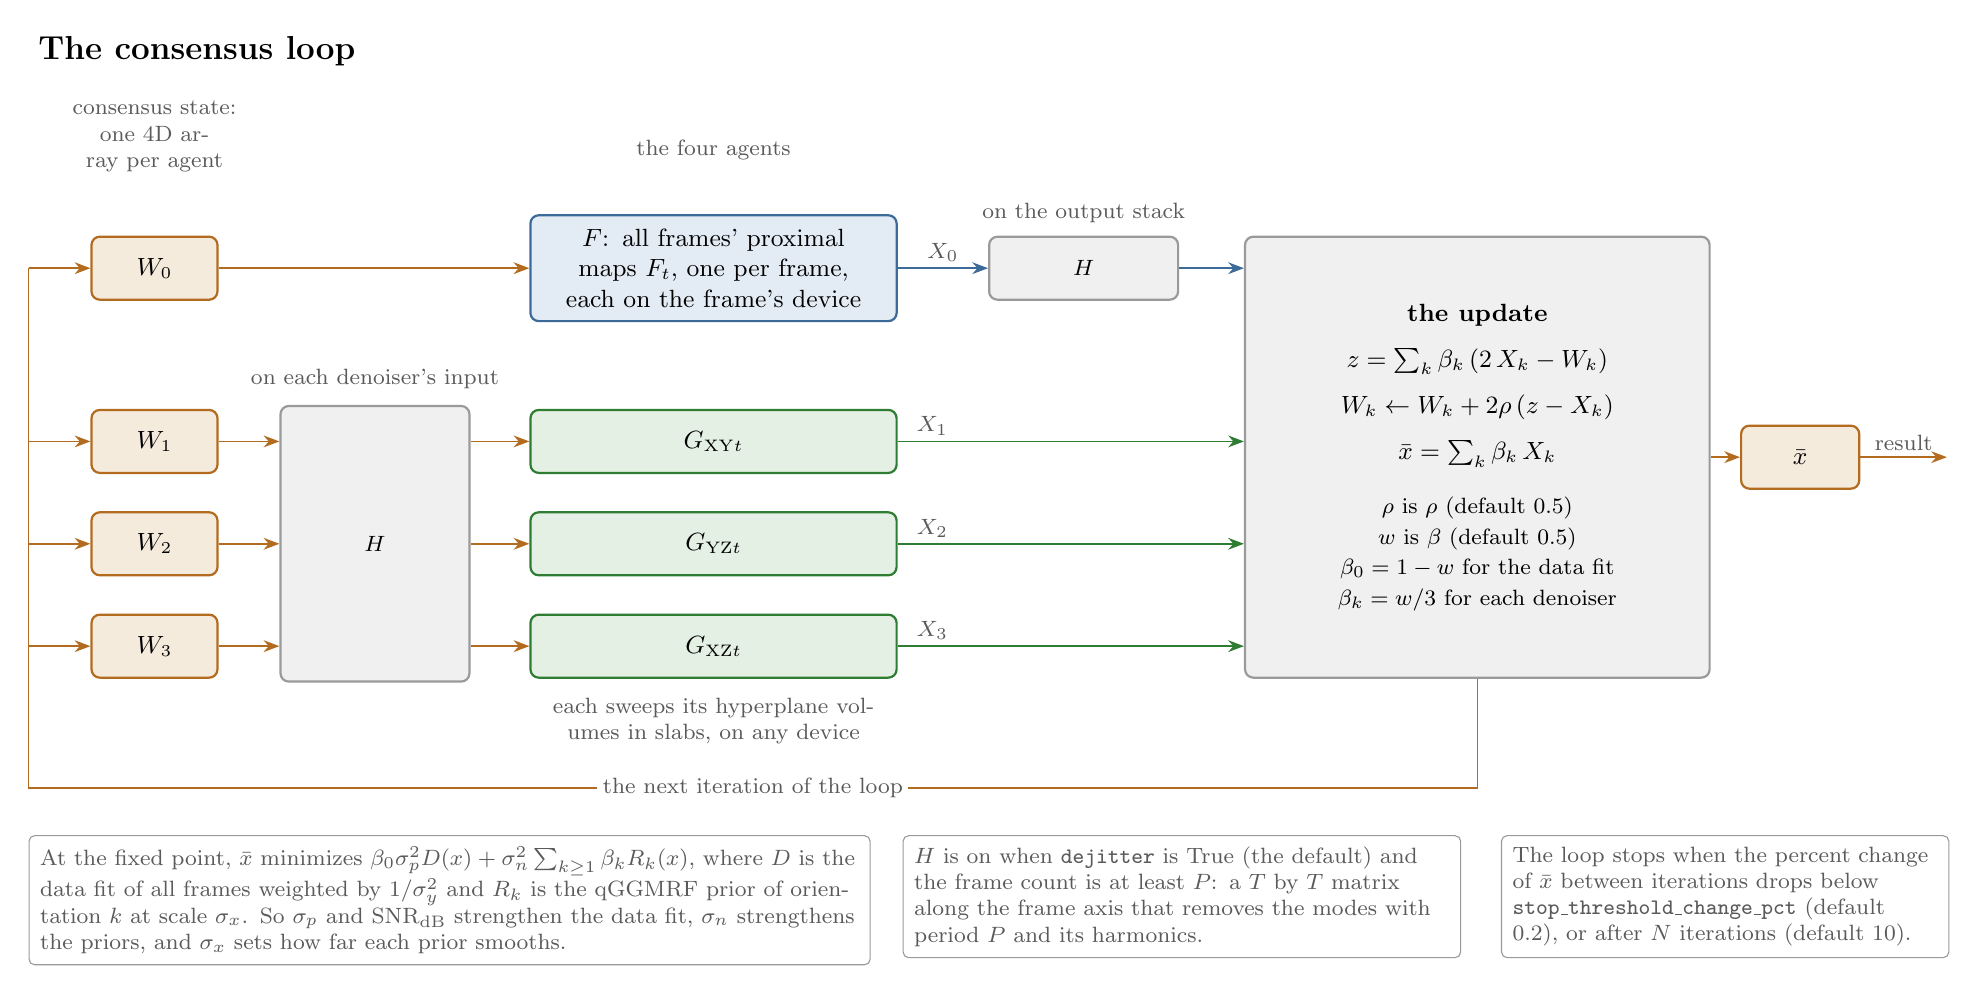
\begin{tikzpicture}[x=1cm, y=1cm]

% ------------------------------------------------------------------ title
\node[title, anchor=west] at (-0.8, 0.55) {\large The consensus loop};

% ------------------------------------------- the consensus state, one per agent
\node[note, anchor=south, align=center, text width=2.7cm] at (0.8, -1.1)
  {consensus state:\\ one 4D array per agent};
\node[state, minimum width=1.6cm] (wzero)  at (0.8, -2.2) {\stateW{0}};
\node[state, minimum width=1.6cm] (wone)   at (0.8, -4.4) {\stateW{1}};
\node[state, minimum width=1.6cm] (wtwo)   at (0.8, -5.7) {\stateW{2}};
\node[state, minimum width=1.6cm] (wthree) at (0.8, -7.0) {\stateW{3}};

% ------------------------------------------------------- the temporal filter
\node[plain, font=\footnotesize, minimum width=2.4cm, minimum height=3.5cm]
  (filterin) at (3.6, -5.7) {\symFilterMatrix};
\node[note, anchor=south] at (3.6, -3.85) {on each denoiser's input};
\node[plain, font=\footnotesize, minimum width=2.4cm]
  (filterout) at (12.6, -2.2) {\symFilterMatrix};
\node[note, anchor=south] at (12.6, -1.75) {on the output stack};

% ------------------------------------------------------------- the four agents
\node[note, anchor=south] at (7.9, -0.95) {the four agents};
\node[datafit, text width=4.3cm] (agentzero) at (7.9, -2.2)
  {\dataFitAgent{}: all frames' proximal maps \proxAgent{t}, one per frame, each on the frame's device};
\node[prior, minimum width=4.65cm] (agentone)   at (7.9, -4.4) {\denoiser{\orientXY}};
\node[prior, minimum width=4.65cm] (agenttwo)   at (7.9, -5.7) {\denoiser{\orientYZ}};
\node[prior, minimum width=4.65cm] (agentthree) at (7.9, -7.0) {\denoiser{\orientXZ}};
\node[note, align=center, text width=7.6cm] at (7.9, -7.95)
  {each sweeps its hyperplane volumes in slabs, on any device};

% ------------------------------------------------------------- the update block
\node[plain, minimum width=5.9cm, minimum height=5.6cm] (update) at (17.6, -4.6)
  {\textbf{the update}\\[2mm]
   $\avgZ = \sum_k \symBeta{k}\,(2\,\outX{k} - \stateW{k})$\\[2mm]
   $\stateW{k} \leftarrow \stateW{k} + 2\symRho\,(\avgZ - \outX{k})$\\[2mm]
   $\xbar = \sum_k \symBeta{k}\,\outX{k}$\\[3mm]
   {\footnotesize $\symRho$ is \pRhoMann{} (default \defRhoMann)}\\
   {\footnotesize $\symPriorWeight$ is \pMacePriorWeight{} (default \defMacePriorWeight)}\\
   {\footnotesize $\symBeta{0} = 1 - \symPriorWeight$ for the data fit}\\
   {\footnotesize $\symBeta{k} = \symPriorWeight/3$ for each denoiser}};

% --------------------------------------------------------------- the result
\node[state, minimum width=1.5cm] (xbar) at (21.7, -4.6) {\xbar};

% ------------------------------------------------- state into the four agents
\draw[flowamber] (wzero.east) -- (agentzero.west);
\draw[flowamber] (wone.east)   -- (filterin.west |- wone.east);
\draw[flowamber] (wtwo.east)   -- (filterin.west |- wtwo.east);
\draw[flowamber] (wthree.east) -- (filterin.west |- wthree.east);
\draw[flowamber] (filterin.east |- agentone.west)   -- (agentone.west);
\draw[flowamber] (filterin.east |- agenttwo.west)   -- (agenttwo.west);
\draw[flowamber] (filterin.east |- agentthree.west) -- (agentthree.west);

% ------------------------------------------- agent outputs into the update
\draw[flowblue] (agentzero.east) -- node[note, above, inner sep=2pt] {\outX{0}} (filterout.west);
\draw[flowblue] (filterout.east) -- (update.west |- filterout.east);
\draw[flowgreen] (agentone.east)   -- node[note, above, inner sep=2pt, pos=0.1] {\outX{1}} (update.west |- agentone.east);
\draw[flowgreen] (agenttwo.east)   -- node[note, above, inner sep=2pt, pos=0.1] {\outX{2}} (update.west |- agenttwo.east);
\draw[flowgreen] (agentthree.east) -- node[note, above, inner sep=2pt, pos=0.1] {\outX{3}} (update.west |- agentthree.east);

% ------------------------------------------------------- the result leaves
\draw[flowamber] (update.east) -- (xbar.west);
\draw[flowamber] (xbar.east) -- node[note, above, inner sep=2pt] {result} ++(1.1,0);

% ------------------------------- the updated state returns for the next pass
\draw[flowamber, -] (update.south) -- (17.6,-8.8) -- (-0.8,-8.8) -- (-0.8,-2.2);
\draw[flowamber] (-0.8,-2.2) -- (wzero.west);
\draw[flowamber] (-0.8,-4.4) -- (wone.west);
\draw[flowamber] (-0.8,-5.7) -- (wtwo.west);
\draw[flowamber] (-0.8,-7.0) -- (wthree.west);
\node[note, fill=white, inner sep=2pt] at (8.4,-8.8) {the next iteration of the loop};

% ------------------------------------------------------------- the notes
\node[notebox, anchor=north west, text width=10.4cm] at (-0.8,-9.4)
  {At the fixed point, \xbar{} minimizes
   $\symBeta{0}\symSigProx^2 D(x) + \symSigNoise^2 \sum_{k \geq 1} \symBeta{k} R_k(x)$,
   where $D$ is the data fit of all frames weighted by $1/\symSigY^2$ and $R_k$ is the
   qGGMRF prior of orientation $k$ at scale $\symSigX$.  So $\symSigProx$ and \pSnrDb{}
   strengthen the data fit, $\symSigNoise$ strengthens the priors, and $\symSigX$ sets
   how far each prior smooths.};
\node[notebox, anchor=north west, text width=6.8cm] at (10.3,-9.4)
  {$\symFilterMatrix$ is on when \pDejitter{} is \defDejitter{} (the default) and the frame
   count is at least \pFramesPerRotation: a $\symNumFrames$ by $\symNumFrames$ matrix along
   the frame axis that removes the modes with period \pFramesPerRotation{} and its harmonics.};
\node[notebox, anchor=north west, text width=5.4cm] at (17.9,-9.4)
  {The loop stops when the percent change of \xbar{} between iterations drops
   below \pStopThreshold{} (default \defStopThreshold), or after \pMaxIterations{}
   iterations (default \defMaxIterations).};

% ---------------------------------------------------- code names and symbols
\ifcodenames
  \node[notebox, anchor=north west, text width=23.7cm] at (-0.8,-11.9)
    {\keyline{\pRhoMann}{\symRho} \hspace{5mm}
     \keyline{\pMacePriorWeight}{\symBeta{k}} \hspace{5mm}
     \keyline{\pSigmaProxMace}{\symSigProx} \hspace{5mm}
     \keyline{\pSigmaNoise}{\symSigNoise} \hspace{5mm}
     \keyline{\pSigmaXMace}{\symSigX} \hspace{5mm}
     \keyline{\filterMatrix}{\symFilterMatrix}};
\fi

\end{tikzpicture}
\end{document}
